\section{\IFRU{Опция TRACE}{TRACE option}}

\TT{TRACE}: \IFRU{трассировать функцию по одной инструкции и сохранять значения всех интересующих нас регистров. После исполнения, эта информация сохранится в файлы process.exe.idc, process.exe.txt, process.exe\_clear.idc. .idc-файлы являются скриптами для IDA, а к .txt файлу можно применять grep, awk, sed для поиска интересующих нас значений.}{trace each instruction in function and collect all interesting values from registers and memory. After execution, all that information is saved to process.exe.idc, process.exe.txt, process.exe\_clear.idc files. .idc-files are IDA scripts, .txt file is grepable by grep, awk and sed.}

\IFRU{Возьмем для примера функцию add\_member из статьи}{For example, let's take add\_member function from} \IT{Using Uninitialized Memory for Fun and Profit}\footnote{\url{http://research.swtch.com/2008/03/using-uninitialized-memory-for-fun-and.html}}\IFRU{}{article}:

\begin{lstlisting}
int dense[256];
int dense_next=0;
int sparse[256];

void add_member(int i)
{
	dense[dense_next]=i;
	sparse[i]=dense_next;
	dense_next++;

};

int main ()
{
	add_member(123);
	add_member(5);
	add_member(71);
	add_member(99);
}
\end{lstlisting}

\IFRU{Скомпилируем и запустим трассировку на функции add\_member (вначале узнайте адрес функции при помощи IDA):}{Let's compile it and run tracing on add\_member function (determine function address in IDA before):}

\begin{lstlisting}
tracer -l:trace_test4.exe bpf=0x00401000,trace:cc
\end{lstlisting}

\IFRU{Получим файл trace\_test4.exe.txt:}{We'll get trace\_test4.exe.txt file:}

\begin{lstlisting}
0x401000, e=       4
0x401001, e=       4
0x401003, e=       4, [0x403818]=0..3
0x401008, e=       4, [EBP+8]=5, 0x47('G'), 0x63('c'), 0x7b('{')
0x40100b, e=       4, ECX=5, 0x47('G'), 0x63('c'), 0x7b('{')
0x401012, e=       4, [EBP+8]=5, 0x47('G'), 0x63('c'), 0x7b('{')
0x401015, e=       4, [0x403818]=0..3
0x40101a, e=       4, EAX=0..3
0x401021, e=       4, [0x403818]=0..3
0x401027, e=       4, ECX=0..3
0x40102a, e=       4, ECX=1..4
0x401030, e=       4
0x401031, e=       4, EAX=0..3
\end{lstlisting}

\IFRU{Поле \IT{e} - это сколько раз была исполнена эта инструкция.}{\IT{e} field is how many times was executed this instruction.}

\IFRU{Загрузим trace\_test4.exe.idc в IDA и увидим:}{Let's execute trace\_test4.exe.idc script in IDA and we'll see:}

\begin{figure}[ht!]
\centering
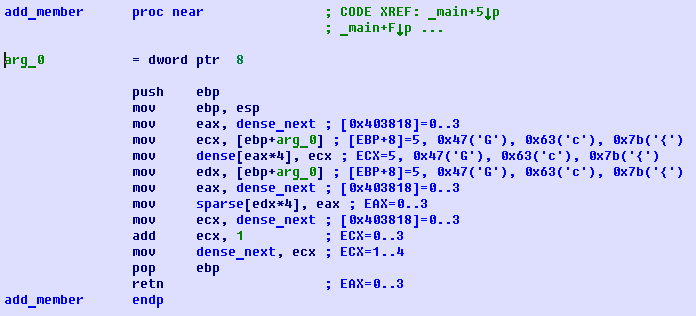
\includegraphics[scale=0.66]{trace_test4.png}
\caption{trace\_test4.png}
\end{figure}

\IFRU{Понимать работу функции во время исполнения, таким образом, становится намного проще.}{Now it is much simpler to understand how this function work during execution.}

\IFRU{Исполненные инструкции подсвечиваются голубым цветом. Неисполненные остаются белыми.}{Executed instructions are highlighed by blue color. Not-executed instructions are leaved white.}

\IFRU{Чтобы стереть все комментарии и подсветку, нужно исполнить скрипт trace\_test4.exe\_clear.idc}{If you need to clear all comments and highlight, execute trace\_test4.exe\_clear.idc script.}

\IFRU{Информация в IDA-скрипте может приводится в сокращенной форме из-за того что IDA имеет ограничение на длину комментария, например: \TT{EAX=[ 64 unique items. min=0xbca6eb7, max=0xffffffed ]}. В текстовом же файле сохраняется всё, поэтому иногда этот файл может оказаться в итоге очень большим.}{All collected information in IDA-script may be reduced to shorten form like \IT{EAX=[ 64 unique items. min=0xbca6eb7, max=0xffffffed ]} (because IDA has comment size limitation). On contrary, everything is saved to text file without shortening, that is why resulting text file may be sometimes pretty big.}

\IFRU{Недостаток опции TRACE в том что она работает медленно, хотя и функции в системных DLL пропускаются (системной считается та DLL которая находится внутри \%SystemRoot\%) Вторая проблема в том что пока что не очень корректно трассируются вещи вроде исключений, setjmp/longjmp и подобных непредвиденных изменений пути исполнения кода.}{One problem of TRACE feature that it is slow, however, functions from system DLLs are skipped (system DLL is that DLL residing in \%SystemRoot\%) Another problem is that things like exceptions, setjmp/longjmp and other unexpected codeflow alterations are not correctly handled so far.}

